\documentclass[a4paper]{report}
\usepackage{algorithmic}
\usepackage{array}
\usepackage{url,amsfonts,amsmath,amssymb,amsthm,color,enumerate,tikz,hyperref}
\usepackage{algorithm,bbm}
\usepackage{mathtools}
% \usepackage{indentfirst}
\usepackage{stackrel}
\usepackage{listings}
\usepackage{subfigure}
\usepackage{subfloat}
\usepackage[justification=centering]{caption}
\usepackage{booktabs} % for three-line table
% \usepackage{subfig}
\usepackage{graphicx}
\setcounter{tocdepth}{4}
\setcounter{secnumdepth}{4}

\hyphenation{op-tical net-works semi-conduc-tor}
\usetikzlibrary{shapes, shadows, arrows}
% \usepackage[english]{babel}
% \usepackage[utf8]{inputenc}
% \usepackage{amsmath}
% \usepackage{graphicx}
% \usepackage[colorinlistoftodos]{todonotes}

\title{Get Start with gr-cdma}

\author{Yu Wang\\umwangyu@umich.edu}

\date{\today}

% def some function
\DeclarePairedDelimiter\ceil{\lceil}{\rceil}
\DeclarePairedDelimiter\floor{\lfloor}{\rfloor}

\newcommand{\specialcell}[2][c]{%
  \begin{tabular}[#1]{@{}c@{}}#2\end{tabular}}

\begin{document}
\maketitle
\tableofcontents
\newpage




% \chapter{Introduction}
\section{What is gr-cdma}
Project gr-cdma is the physical layer of CDMA communication. This project is developed based on GNURadio\cite{GNURadio}.
gr-cdma is created and maintained by Prof. Anastasopoulos.
The whole source codes are on github \url{https://github.com/anastas/gr-cdma}.
This project is to build a communication block which employs DS-CDMA technique to build the link.
The user does not have to know the details of the schemes, but could transmit reliably through this physical layer protocol.

\section{What is GNURadio}
GNURadio\cite{GNURadio} is a open-source *unix based platform which enables developers and researchers design and test their self-built communication or signal processing system.
The whole platform is written by c++. Developer could use c++ or python to customize their own block. gr-cdma is a customized block as well.

\section{What is the Current State of gr-cdma}
Till 17-Jun-2016, the main part of this project is finished.
The next step is to optimize the working strategy for several block to make the system more robust in field test. 
This document is an introduction of what this project is, how to get start with GNURadio and gr-cdma and what are the issues to be solved. 
\chapter{Introduction}
\section{What is gr-cdma}
Project gr-cdma is the physical layer of CDMA communication. This project is developed based on GNURadio\cite{GNURadio}.
gr-cdma is created and maintained by Prof. Anastasopoulos.
The whole source codes are on github \url{https://github.com/anastas/gr-cdma}.
This project is to build a communication block which employs DS-CDMA technique to build the link.
The user does not have to know the details of the schemes, but could transmit reliably through this physical layer protocol.

\section{What is GNURadio}
GNURadio\cite{GNURadio} is a open-source *unix based platform which enables developers and researchers design and test their self-built communication or signal processing system.
The whole platform is written by c++. Developer could use c++ or python to customize their own block. gr-cdma is a customized block as well.

\section{What is the Current State of gr-cdma}
Till 17-Jun-2016, the main part of this project is finished.
The next step is to optimize the working strategy for several block to make the system more robust in field test. 
This document is an introduction of what this project is, how to get start with GNURadio and gr-cdma and what are the issues to be solved. 



% \chapter{Working Strategy of gr-cdma}
In this chapter, we will discuss the working strategy of gr-cdma, the principle of each main block.
Mathematic models and analyses are involved to describe the situation.

\section{The diagram of The Tx \& Rx}
Here are the digrams for Tx and Rx. 
\begin{figure}[!ht]
	\centering
	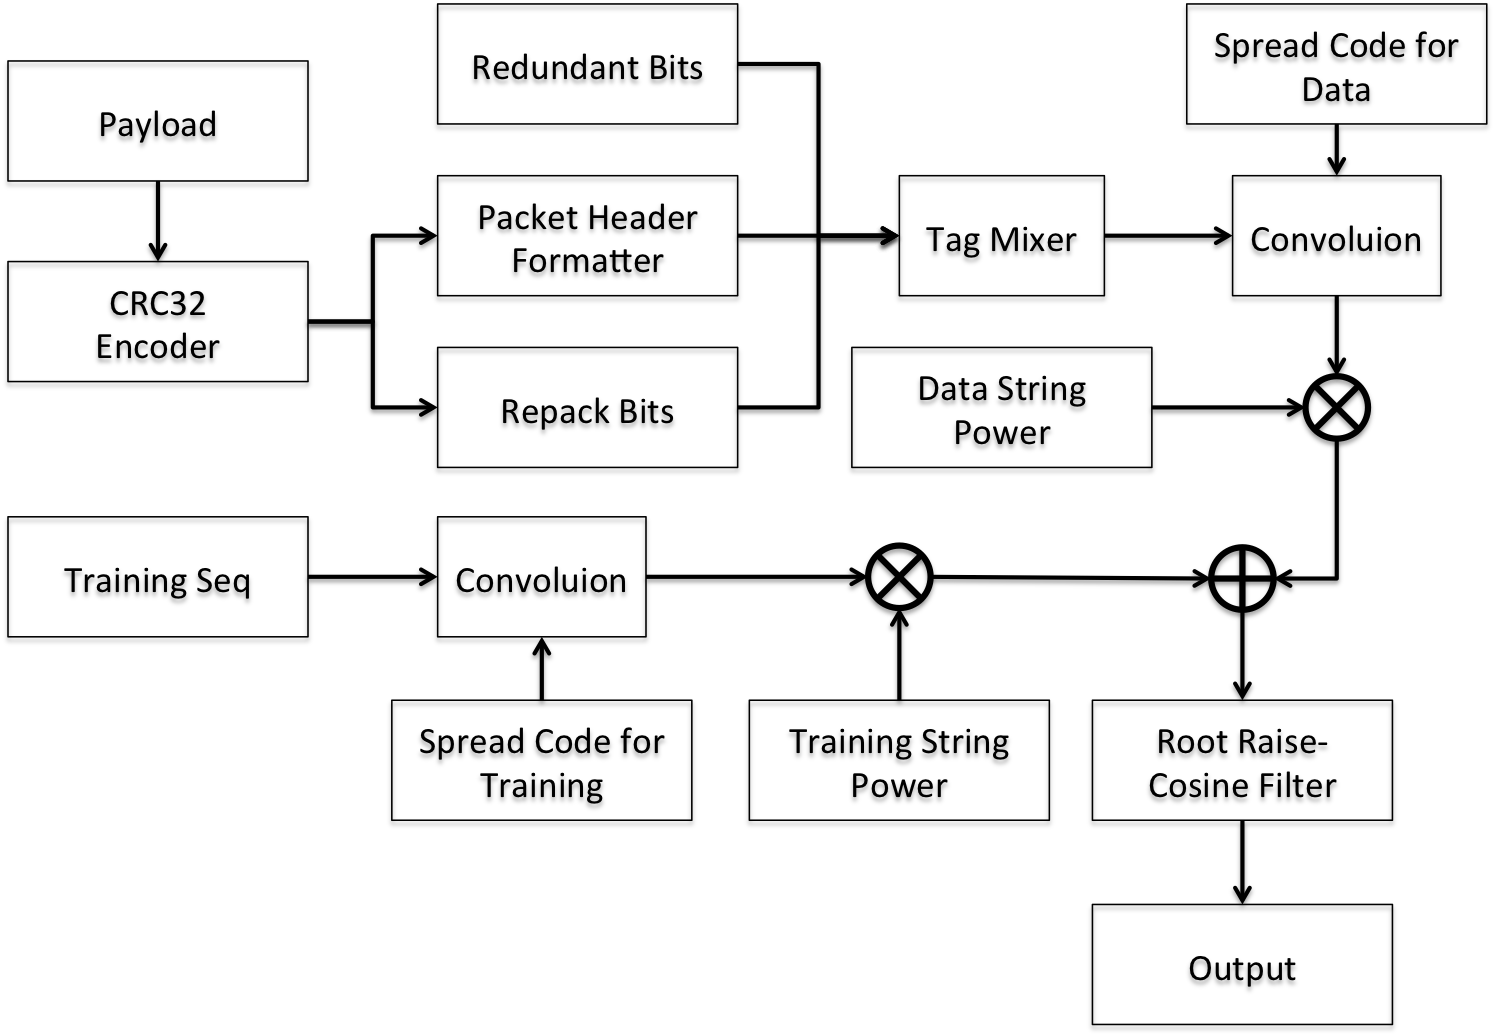
\includegraphics[width = 5 in]{figure/tx-diagram.png}
	\caption{Diagram for Tx}
	\label{fig:diagram for Tx}
\end{figure}
\begin{figure}[!ht]
	\centering
	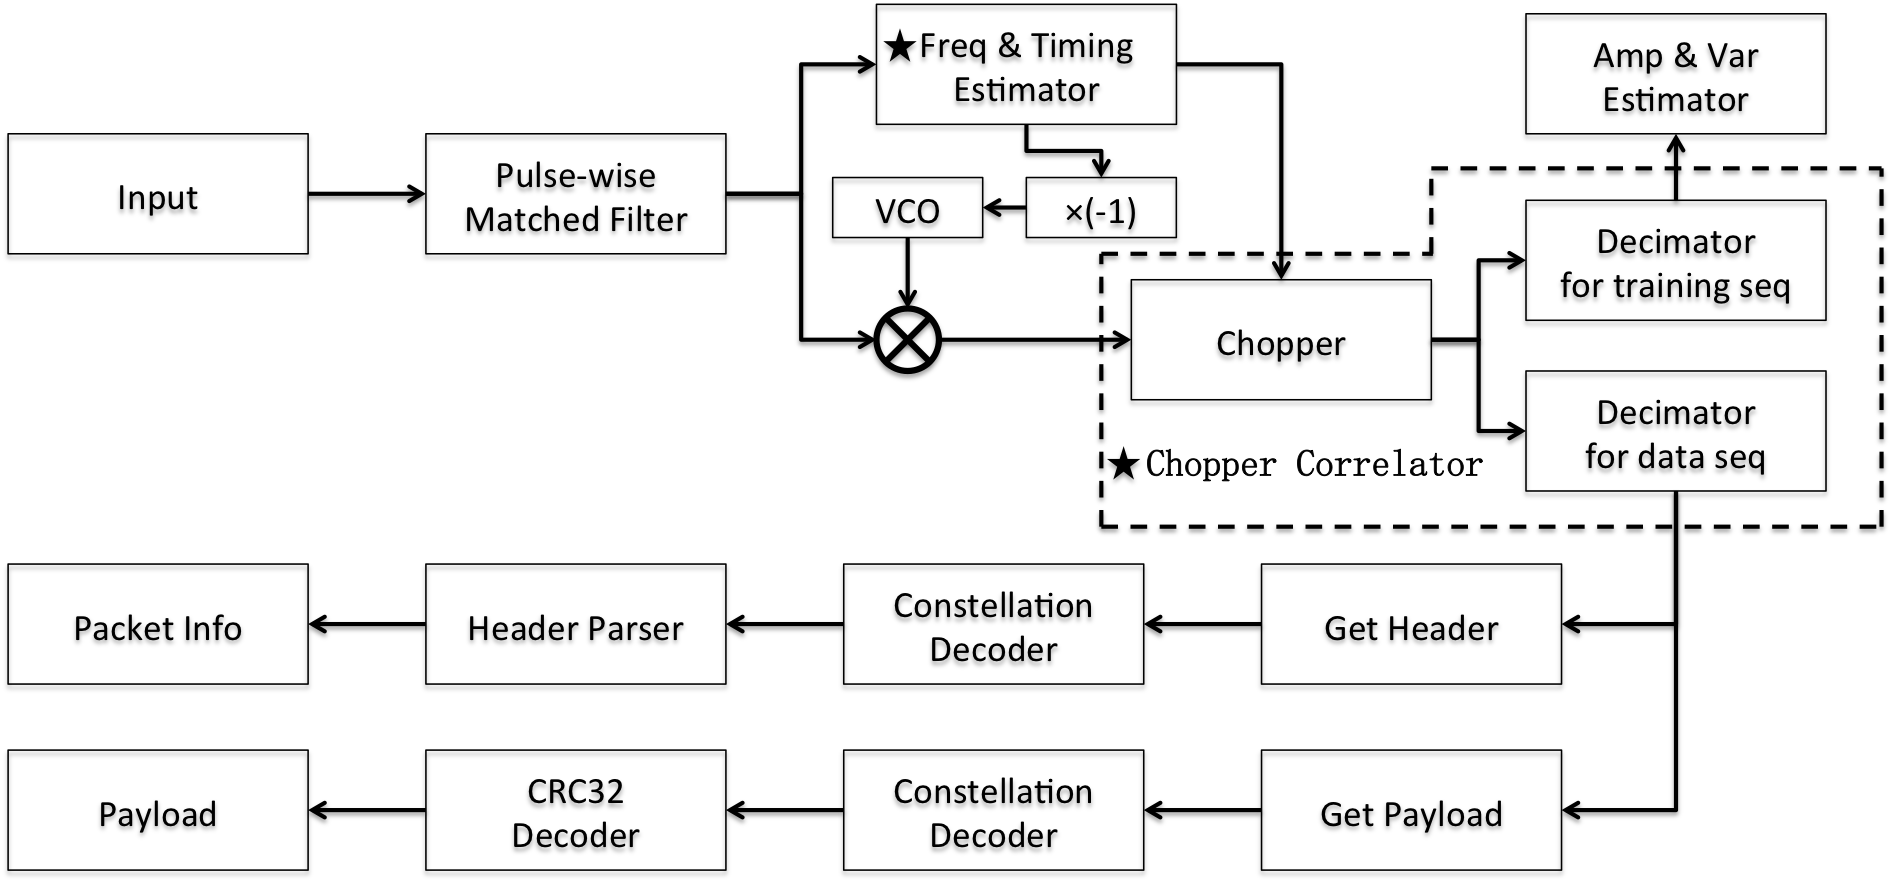
\includegraphics[width = 5in]{figure/rx-diagram.png}
	\caption{Diagram for Rx}
	\label{fig:diagram for Rx}
\end{figure}

From fig \ref{fig:diagram for Tx} and fig \ref{fig:diagram for Rx}, you may find that the system is a little bit more complicated than you thought. And also, the receiver is bigger than the transmitter. In fact, it is for the reason that the receiver will deal with no only the decoding part, but also the synchronization problem. which is actually the most difficult part for this system.

\section{Transmitter} % (fold)
\label{sec:transmitter}
The duty for transmitter is to package the payload or the input data, build the packet structure, generate the training sequence, modify the power for each section and form the waveform. Similar to other CDMA system, one of the essential part of the system is about the spreading code. The quality of the spreading code will affect greatly about the performance of synchronization parts. Intuitively, we would like to use codes like m-sequences and gold sequence, which has high auto-correlation and flat cross-correlation value.

\begin{figure}
	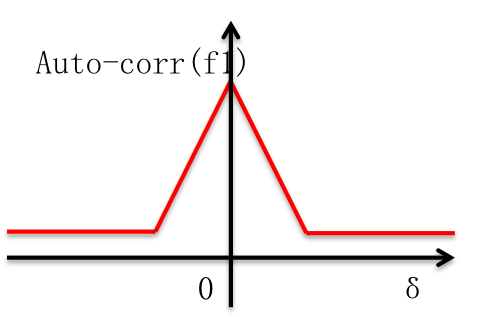
\includegraphics[width = 3in]{figure/bad_correlation.png}
	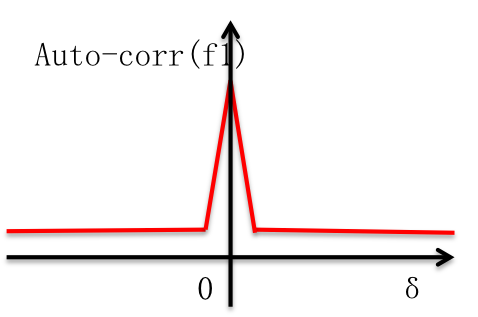
\includegraphics[width = 3in]{figure/good_correlation.png}
\end{figure}

% section transmitter (end)
\chapter{Working Strategy of gr-cdma}
In this chapter, we will discuss the working strategy of gr-cdma, the principle of each main block.
Mathematic models and analyses are involved to describe the situation.

\section{The diagram of The Tx \& Rx}
Here are the digrams for Tx and Rx. 
\begin{figure}[!ht]
	\centering
	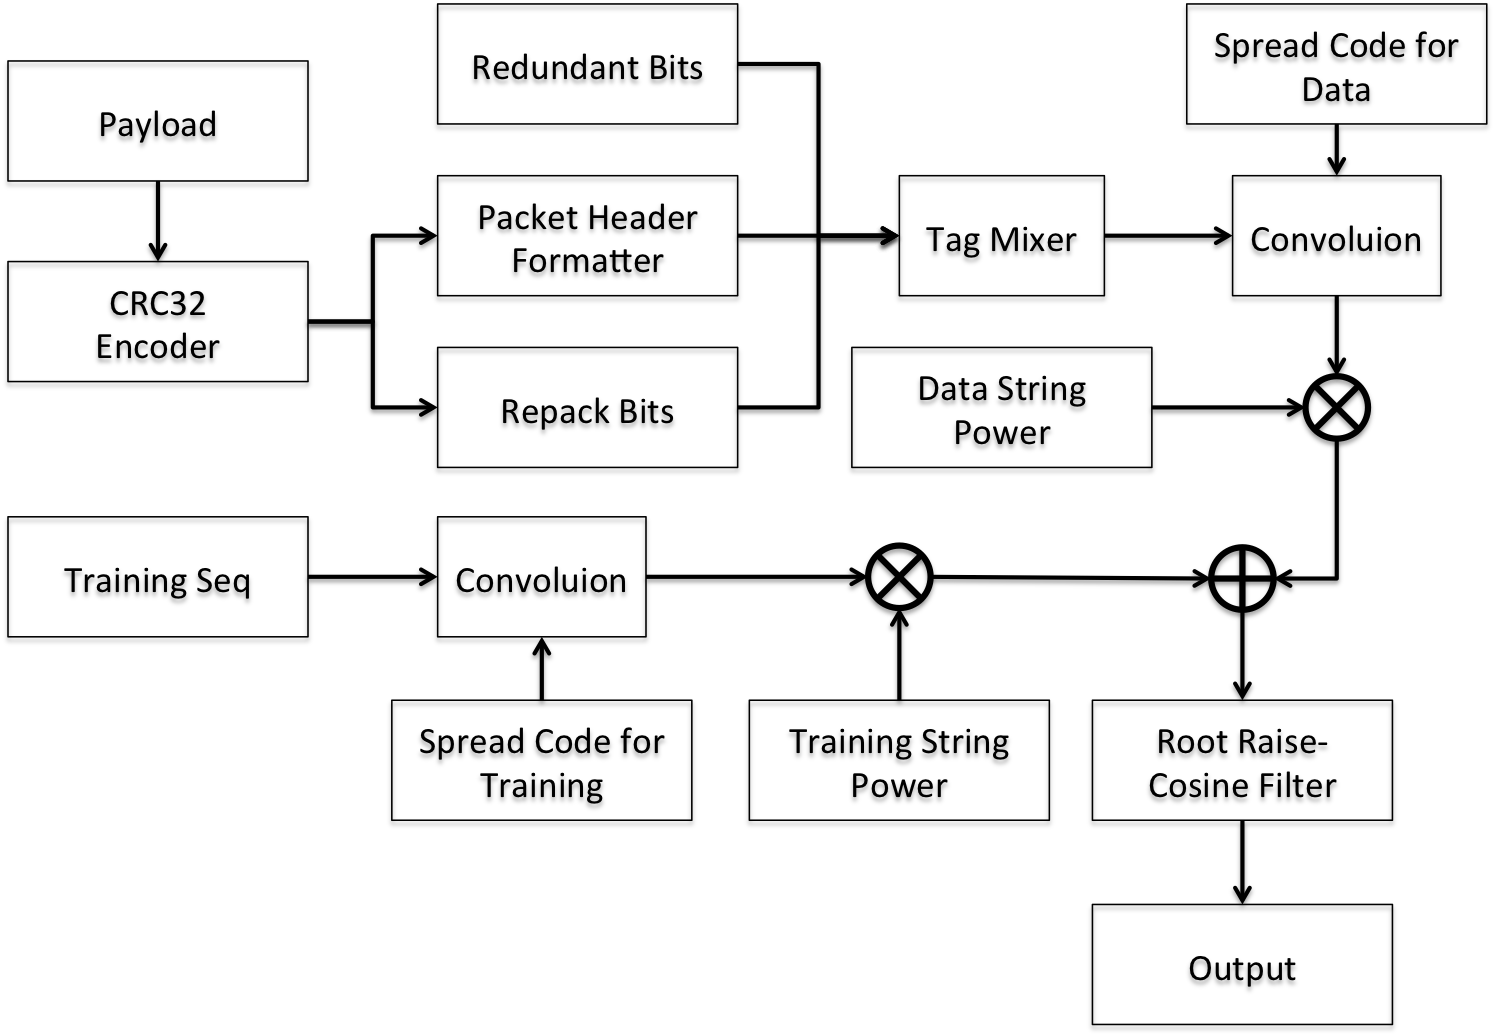
\includegraphics[width = 5 in]{figure/tx-diagram.png}
	\caption{Diagram for Tx}
	\label{fig:diagram for Tx}
\end{figure}
\begin{figure}[!ht]
	\centering
	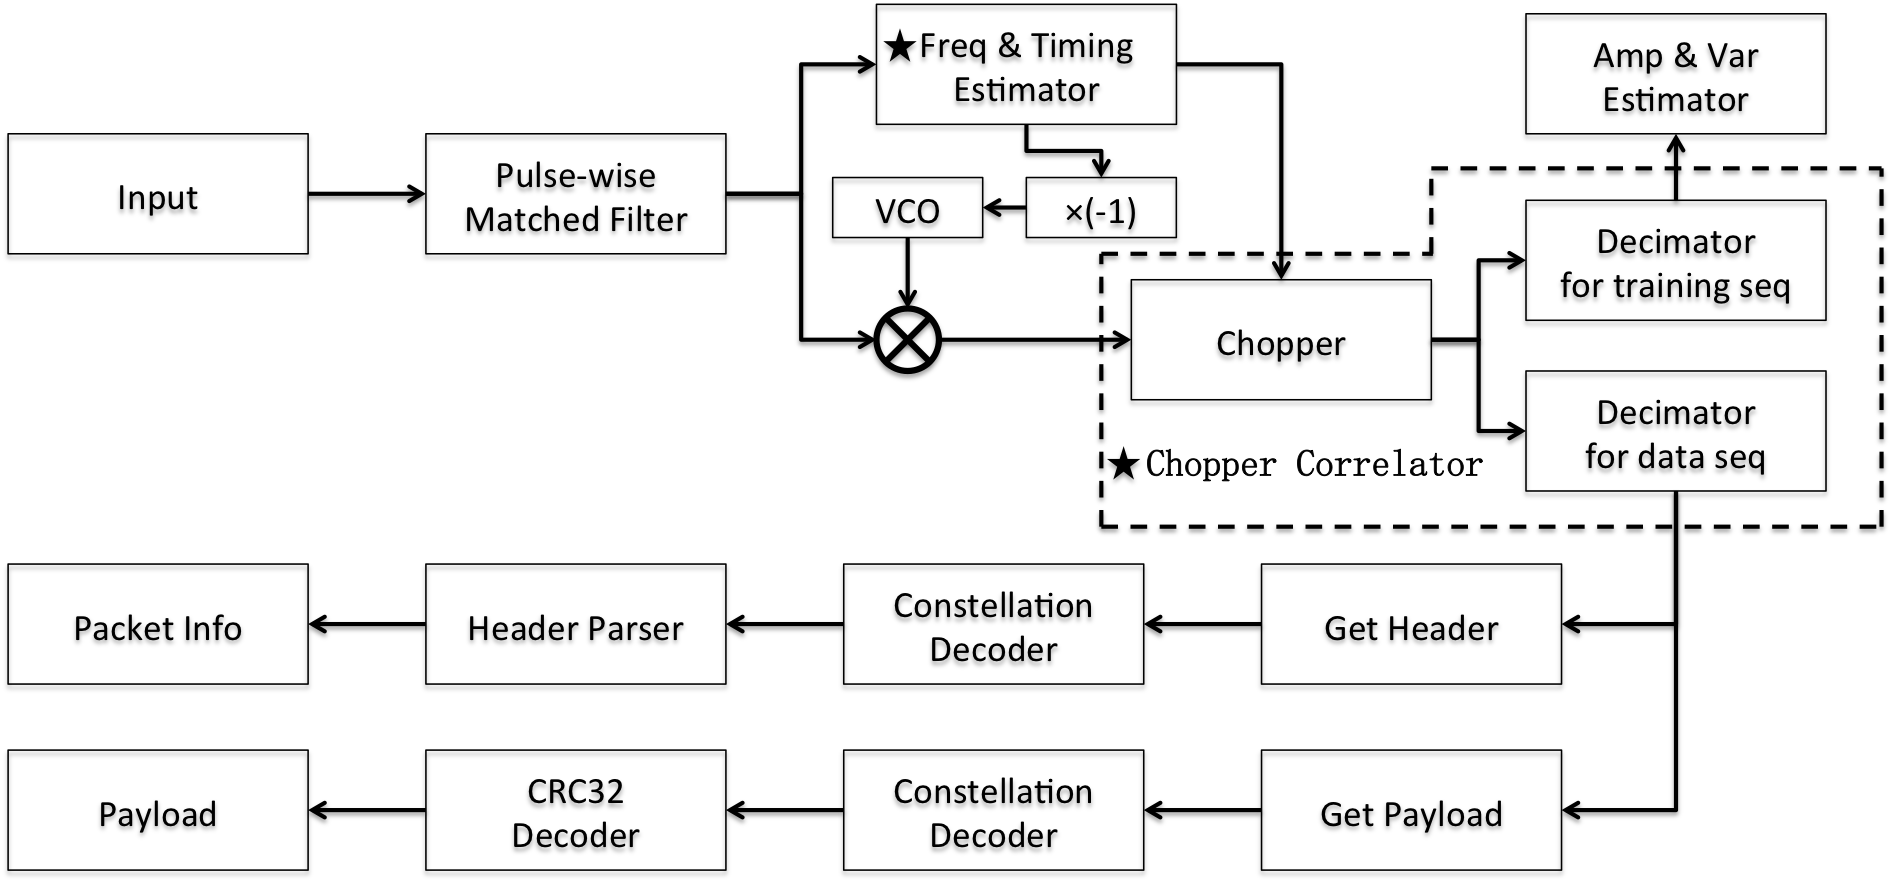
\includegraphics[width = 5in]{figure/rx-diagram.png}
	\caption{Diagram for Rx}
	\label{fig:diagram for Rx}
\end{figure}

From fig \ref{fig:diagram for Tx} and fig \ref{fig:diagram for Rx}, you may find that the system is a little bit more complicated than you thought. And also, the receiver is bigger than the transmitter. In fact, it is for the reason that the receiver will deal with no only the decoding part, but also the synchronization problem. which is actually the most difficult part for this system.

\section{Transmitter} % (fold)
\label{sec:transmitter}
The duty for transmitter is to package the payload or the input data, build the packet structure, generate the training sequence, modify the power for each section and form the waveform. 

\subsection{Spreading Code} % (fold)
\label{sub:spreading_code}

Similar to other CDMA system, one of the essential part of the system is about the spreading code. The quality of the spreading code will affect greatly about the performance of synchronization parts. Intuitively, we would like to use codes like m-sequences and gold sequence, which has high auto-correlation and flat cross-correlation value.

\begin{figure}
	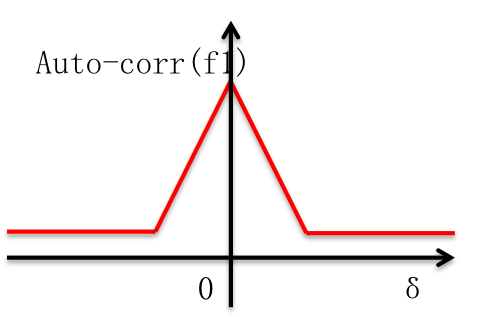
\includegraphics[width = 3in]{figure/bad_correlation.png}
	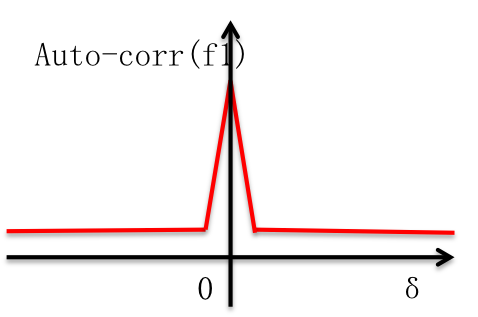
\includegraphics[width = 3in]{figure/good_correlation.png}
\end{figure}

The most famous spreading code is the m-sequence. 
\subsubsection{M-Sequence} % (fold)
\label{ssub:m_sequence}

M-sequence is a kind of sequnece with very good property. for m-sequnece $p(k)$, 
\begin{align}
	p(k) \ast p(k+\delta_k) = 
	\begin{cases}
	m    & \delta_k = 0\\
	-1	 & \delta_k \neq 0
	\end{cases}
\end{align}
$m$ is the length of sequence, $\delta_k$ ranges from $-m+1$ to $m-1$.

Here is the table for some m-sequence, table \ref{tab:M-sequence feedback connections generated using LFSR generator}

\begin{table}[ht]
\centering
\caption{M-sequence feedback connections generated using LFSR generator}
\label{tab:M-sequence feedback connections generated using LFSR generator}
\begin{tabular}{c c c c}
\hline
\begin{tabular}[c]{@{}l@{}}Number \\ of shift \\ registers,\\  $L$\end{tabular} & \begin{tabular}[c]{@{}l@{}}Code \\ length \\ $N_c = 2^l-1$\end{tabular} & Feedback Taps for M-sequence & \begin{tabular}[c]{@{}l@{}}No. of \\ M-sequence \\ codes\end{tabular} \\ \hline
2 & 3 & {[}2,1{]} & 1 \\ 
3 & 7 & {[}3,2{]} & 2 \\ 
4 & 15 & {[}4,1{]} & 2 \\ 
5 & 31 & {[}5,3{]}, {[}5,4,3,2{]}, {[}5,4,2,1{]} & 6 \\ 
6 & 63 & {[}6,1{]}, {[}6,5,2,1{]}, {[}6,5,3,2{]} & 6 \\ 
7 & 127 & \begin{tabular}[c]{@{}l@{}}{[}7,1{]}, {[}7,3{]},{[}7,3,2,1{]}, {[}7,4,3,2{]}, {[}7,6,4,2{]}, \\ {[}7,6,3,1{]}, {[}7,6,5,2{]}, {[}7,6,5,4,2,1{]}, \\ {[}7,5,4,3,2,1{]}\end{tabular} & 18 \\ 
8 & 255 & \begin{tabular}[c]{@{}l@{}}{[}8,4,3,2{]}, {[}8,6,5,3{]}, {[}8,6,5,2{]}, {[}8,5,3,1{]}, \\ {[}8,6,5,1{]}, {[}8,7,6,1{]}, {[}8,7,6,5,2,1{]}, \\ {[}8,6,4,3,2,1{]}\end{tabular} & 16 \\ 
9 & 511 & \begin{tabular}[c]{@{}l@{}}{[}9,4{]}, {[}9,6,4,3{]}, {[}9,8,5,4{]}, {[}9,8,4,1{]}, \\ {[}9,5,3,2{]}, {[}9,8,6,5{]}, {[}9,8,7,2{]}, \\ {[}9,6,5,4,2,1{]}, {[}9,7,5,3,1{]}, {[}9,8,7,6,5,3{]}\end{tabular} & 48 \\ 
10 & 1023 & \begin{tabular}[c]{@{}l@{}}{[}10,3{]}, {[}10,8,3,2{]}, {[}10,4,3,1{]}, {[}10,8,5,1{]}, \\ {[}10,8,5,4{]}, {[}10,9,4,1{]}, {[}10,8,4,3{]}, \\ {[}10,5,3,2{]}, {[}10,5,2,1{]}, {[}10,9,4,2{]}, \\ {[}10,6,5,3,2,1{]}, {[}10,9,8,6,3,2{]}, \\ {[}10,9,8,7,6,5,4,3{]}, {[}10,8,7,6,5,4,3,1{]}\end{tabular} & 176 \\ \hline
\end{tabular}
\end{table}

% subsection m_sequence (end)
\subsubsection{Gold Sequence} % (fold)
\label{sub:gold_sequence}

But also as shown in the table above, the number of m-sequence for certain length is not that much. So, some other sequences like ``Gold sequences'' are generated. ``Gold sequence'' is actually the shift-add of two m-sequence. When the shift space for tow m-sequence is different, more relatively good sequences are generated.

% subsubsection gold_sequence (end)

\subsubsection{Spreading Seuquence used in gr-cdma} % (fold)
\label{ssub:short_seuquence}

But for gr-cdma, we adopt sequence of length 8. From the diagram, we know that a functioning system needs two spreading sequences for ``Training'' and ``Data''. So we only need two relatively good sequences. Because the length of codes are not long enough, so brutal search is feasible. 
For current system, the two sequences are as shown in table \ref{tab:Spread Codes for gr-cdma}

\begin{table}[ht]
 	\centering
 	\caption{Spread Codes for gr-cdma}
 	\label{tab:Spread Codes for gr-cdma}
 	\begin{tabular}{c c}
 	\hline
 		Type of Sequence 	& 	Sequence \\ \hline
 		Training Sequence 	& 	[+1, +1, +1, +1, -1, +1, +1, -1]\\ 
 		Data Sequence 		& 	[-1, +1, -1, +1, -1, -1, -1, -1]\\ \hline
 	\end{tabular}
 \end{table} 
% subsubsection short_seuquence (end)

% subsection spreading_code (end)

\subsection{Packet Structure} % (fold)
\label{sub:packet_structure}

Packeting is also one main part for Transmitter. In physical layer, transmitting purely meaningless 0s and 1s reliably and efficiently is good. But for a system, we may care the index of each sequence, which is good for placing different pieces in order, modulation scheme, adaptive modulations may be used, and so on. The training and data packet structure for gr-cdma is like figure \ref{fig:training_frame} and figure \ref{fig:data_frame}:
\begin{figure}[ht]
	\centering
	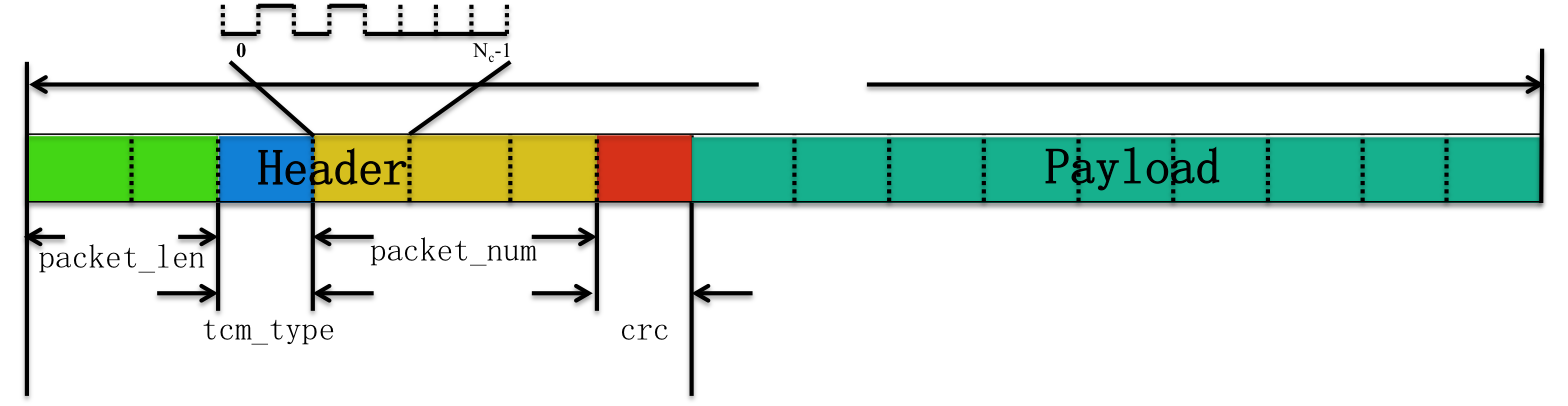
\includegraphics[width = 5in]{figure/data_frame.png}
	\caption{Data Frame}
	\label{fig:data_frame}
\end{figure}
\begin{figure}[ht]
	\centering
	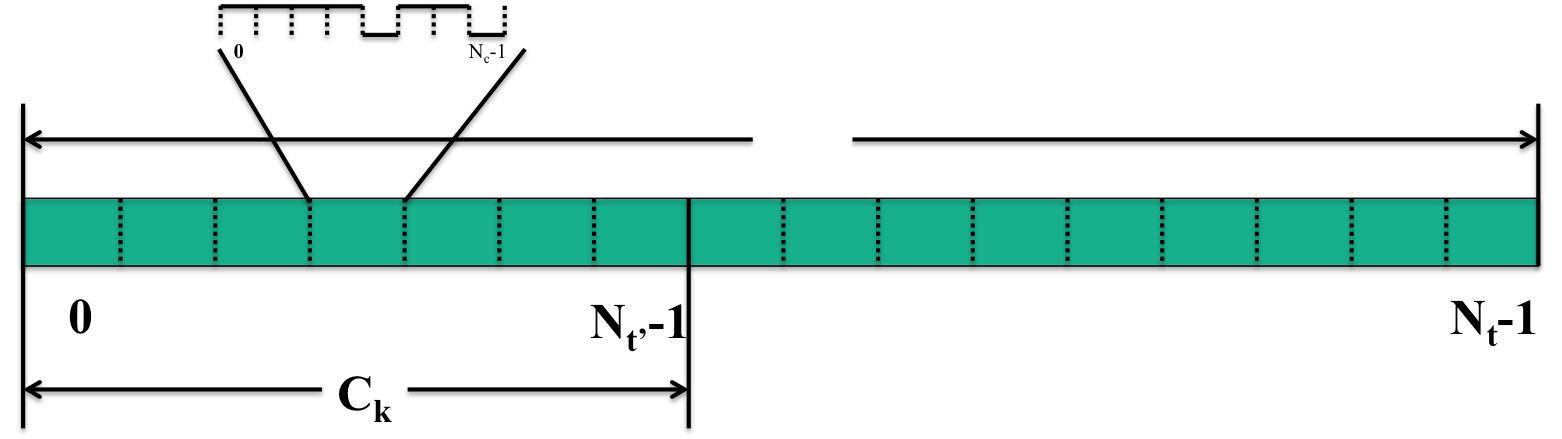
\includegraphics[width = 5in]{figure/training_frame.png}
	\caption{Training Frame}
	\label{fig:training_frame}
\end{figure}

In current version, because the number of binary bits for each Segment of the frame is set through ``python/cdma\_parameter.py'', the length for these part is 
\begin{table}[ht]
	\centering
	\caption{Length for Each Part of Frame}
	\label{tab:Length_for_each_part_of_frame}
	\begin{tabular}{c c c}
	\hline
		Frame Type 	& Segment Type 	& Segment Length\\ \hline
		Training 	& /		 		& 260			\\
		Data 		& packet length & 12 			\\
		Data 		& tcm type 		& 4 			\\
		Data 		& packet index 	& 16 			\\
		Data 		& header crc 	& 8 			\\ \hline
	\end{tabular}
\end{table}
% subsection packet_structure (end)

\subsection{Power Control} % (fold)
\label{sub:power_control}
As shown in the figure \ref{fig:diagram for Tx}, training sequence and data sequence are two separate branches. In reality, the power a transmitter could provide is certain, so before adding them up, the power arrangement should be considered. In ``python/cdma\_parameter.py'', variable ``training\_percent'' is to control the percentage of power used for Training sequence. 
% subsection power_control (end)

\subsection{Multi-Sampling and Pulse Shaping} % (fold)
\label{sub:multi_sampling}
Multi-Sampling is good for synchronization. In modern CDMA communication systems, like GPS, each chip will be sampled twice. Besides, we could not transmit digital signals directly, blocks like Root Raise-Cosine Filter will be added at the end of the block. The parameter set for RRCF is 
\begin{table}[ht]
	\centering
	\caption{Parameters for Root Raise-Cosine Filter}
	\begin{tabular}{cc}
	\hline
		Parameter 			& 	Value 	\\ \hline
		Samples Per Chip 	& 	2 		\\
		The rolloff factor 	& 	0.35 	\\
		Filter length 		& 	21 		\\ \hline
	\end{tabular}
\end{table}
% subsection multi_sampling (end)
% section transmitter (end)

\section{Receiver} % (fold)
\label{sec:receiver}

Comparatively, receiver is more complicated than transmitter. Because in the real time, receiver does not have any knowledge of received signal's time and frequency shift. As shown in the diagram Figure \ref{fig:diagram for Rx},  the most important block for receiver is not the decoding part, but the frequency and timing estimator. The theory for frequency and timing estimator will be shown in detail in Chapter \ref{ch:Mathematic Bases}

\subsection{Frequency and Timing Estimator} % (fold)
\label{sub:frequency_and_timing_estimator}
Frequency and Timing Estimator generally gives the estimation of timing information and frequency shift. We do not design a frequency estimator and timing estimator separately, but together. 
\subsubsection{Timing Information} % (fold)
\label{ssub:timing_information}

In communication system, information bit sequence needs to be packaged with certain structure form. Same as gr-cdma, we also create a certain frame structure. The structure is shown in Figure \ref{fig:Training Frame Structure} and Figure \ref{fig:Data Frame Structure}. When we need to decode them, or say extract the payload from the frame, we need to know ``Where should we start cutting''. We want to remain exactly the information bit sequence, rather than a broken sequence with other ``meaningless'' bits. So, we need to get the start point of each frame. 

The method we use is pretty straight forward. We use another frame called Training Frame. The output signal is the sum of Training and Data. Because we carefully select the spread code for training and data, they will not mass up when added up together. Each training frame are exactly the same. So, we could use a matched filter to find the end point of the frame. Because when the matched filter outputs a peak, it means there exists a potential whole length training frame in the received signal sequence. Thanks to the design that training frame and data frame are perfectly aligned, the ending point for training frame is the same as the ending point for data frame. So, we solve the problem of timing.
% subsubsection timing (end)

\subsubsection{Frequency Information} % (fold)
\label{ssub:frequency_information}

To be precisely, the frequency information we talk here is the frequency shift provided by the channel. In real environment, reasons like clock drift and Doppuler effect can change the received signal's frequency. If the transmitter and receiver's oscillator are not synchronized, the performance will not be that good. So, the receiver will try to find out the frequency difference between the received signal and local oscillator, and narrow the gap as small as possible. 

Frequency estimator share nearly the same idea as timing estimator. It is true that there are many other methods like doing FFT and find out the frequency gap. But as mentioned, we need to do a joint estimation of both timing and frequency. We designed a matched filter bank to deal with this problem.

% subsubsection frequency (end)
\subsubsection{Structure for Joint Estimator} % (fold)

The diagram for Frequency and Timing estimator is shown in Figure \ref{fig:Diagram for Frequency and Timing Estimator}.
\label{ssub:structure_for_joint_estimator}
\begin{figure}[ht]
	\centering
	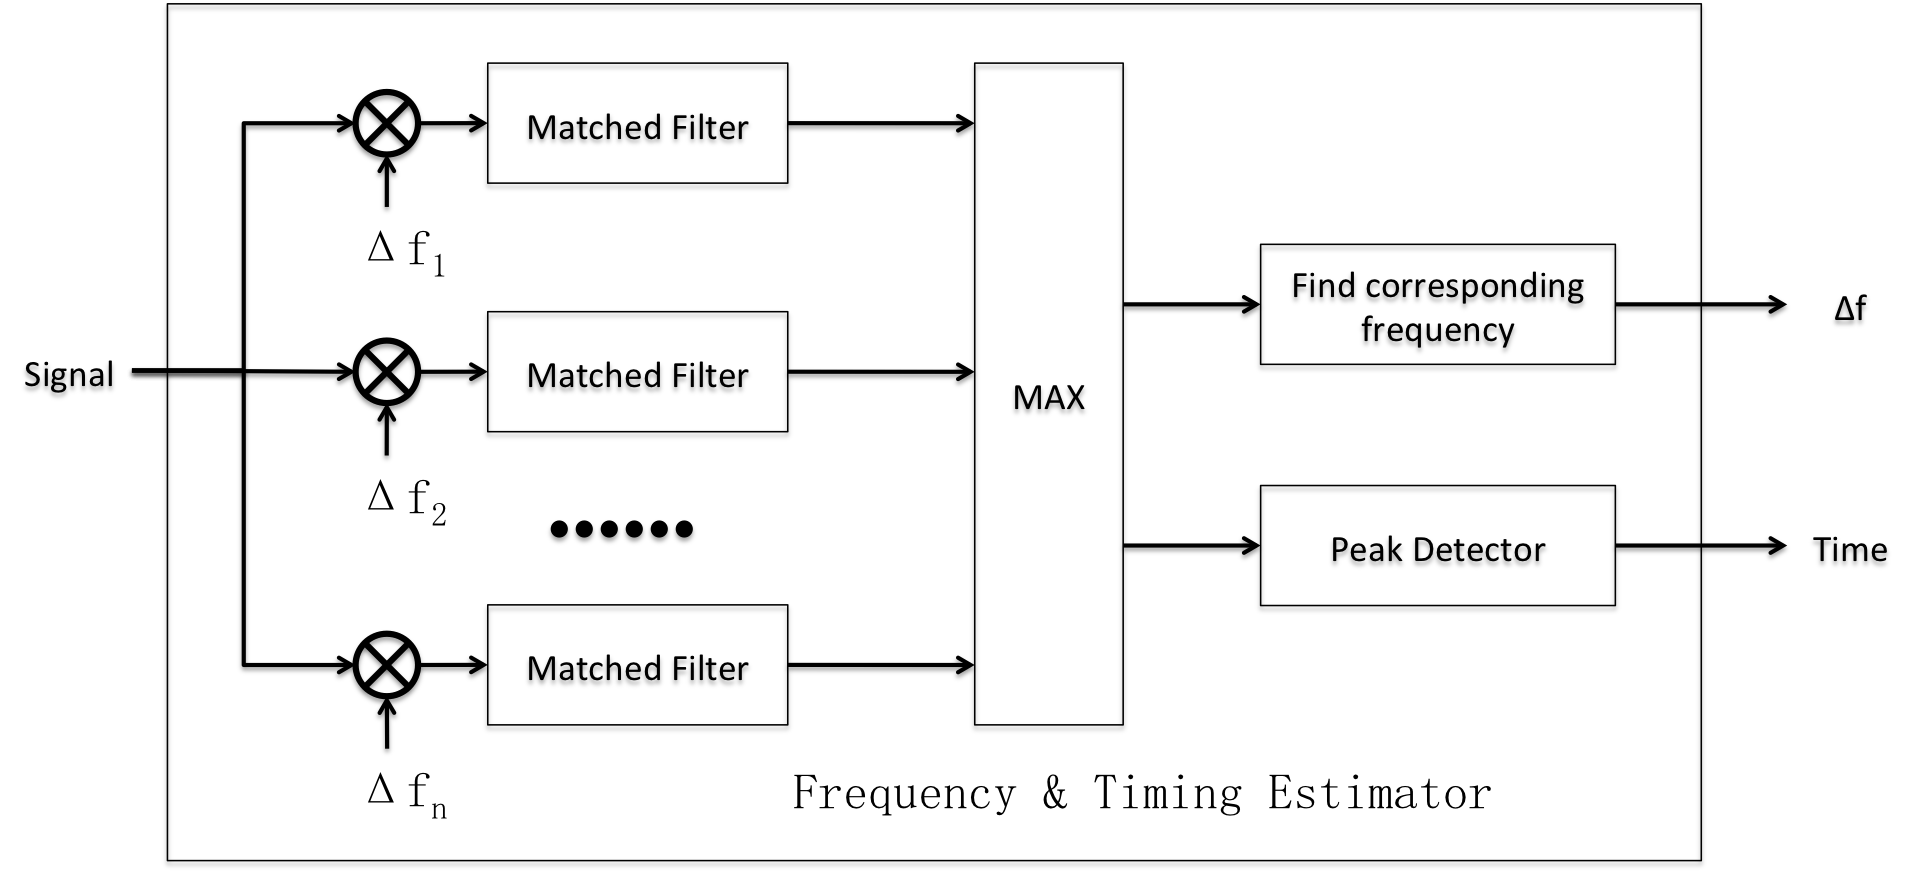
\includegraphics[width = 5in]{figure/frequency_and_timing_estimator_diagram.png}
	\caption{Diagram for Frequency \& Timing Estimator}
	\label{fig:Diagram for Frequency and Timing Estimator}
\end{figure}

In gnuradio, there is a block called ``xlating filter''. It works exactly the same as multiplying a frequency and then do matched filtering. 
\begin{figure}[ht]
	\centering
	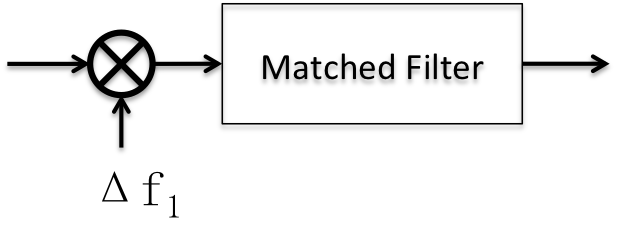
\includegraphics[width = 3in]{figure/xlating_filter_diagram.png}
	\caption{xlating-filter in gnuradio companion}
	\label{fig:xlating filter in gnuradio companion}
\end{figure}

Because there is a large number of matched filter in this block, we need to make this block working as efficiently as it could. We choose to use the FFT version of filter rather than the traditional one.
% subsubsection structure_for_joint_estimator (end)

% subsection frequency_and_timing_estimator (end)

\subsection{De-spreading} % (fold)
\label{sub:De-spreading_strategy}

De-spreading is to demodulate the CDMA signal. The method is straight forward. Use a matched filter which equipped with the patten matching spreading code for training / data, then see whether the peak is positive or negative. Then, sample only at positions where we see peak. 

The block in gnuradio that can do this is called ``decimation''.
% subsection De-spreading_strategy (end)

\subsection{Packet Parser} % (fold)
\label{sub:packet_parser}

Packet Parser only check the header information. In data frame, there is a field called ``CRC''. It the receiver could generate exactly the same CRC as the bits in the CRC field, this frame will be regarded as valid. It is true that, there are cases where the packet is broken, but the CRC happens to be ``Correct''. We have nothing to do with cases of such.
% subsection packet_parser (end)

\subsection{Error Calculator} % (fold)
\label{sub:error_calculator}

This block is to give a rough estimation of packet error rate. The working strategy is as below.

There are two counters. One counter counts the number of packets pass the Packet Parser, which are regard as valid packet. The value for this counter is called $C_{vp}$. Another counter counts the total number of any packets that received in one iteration. This counter's value is called $C_{all}$. This block has one parameter called ``Window Size''. Every time, when $C_{vp} = Window Size$, we will output the ratio $C_{vp} / C_{all}$. But, we should bury in mind that, the Packet Parser will output only the valid packet. So, how do we count $C_{all}$? To solve this problem, we choose a little complicated way. We use the index of each packet. If the packets' indices are consecutive, like $1, 2, 3...$, then we will add $1$, $1$ and $1$ to both $C_{vp}$ and $C_{all}$. But when we miss a packet, we may see indices like $1, 2, 5$, we know that there should have missed $5-2-1 = 2$ packets. But pay attention, the index for packet could not be infinity, there is a limit. If the largest index is $255$, when we see $254, 255, 0$, we should not treat it as nonconsecutive. Also, we need to treat problems when we see $254, 255, 2$. Out solution to treat situations where we face the end of one iteration of index is to add the number of iteration to the index which has already start from 0. When we see $255, 0$, we will add $256$ to 0. So we will deal with sequence $255, 256$, they are consecutive obviously. But the next step would return to deal with $0, 1$, rather than $256, 257$. 
% subsection error_calculator (end)
% section receiver (end)

\chapter{Mathematic Bases}
\label{ch:Mathematic Bases}
\section{Introduction} % (fold)
\label{sec:Introduction}
CDMA system is famous for its large user capacity and superior ability of keeping security. In practical CDMA system, the diagram of the whole system is like 
\begin{figure}[ht]
	\centering
	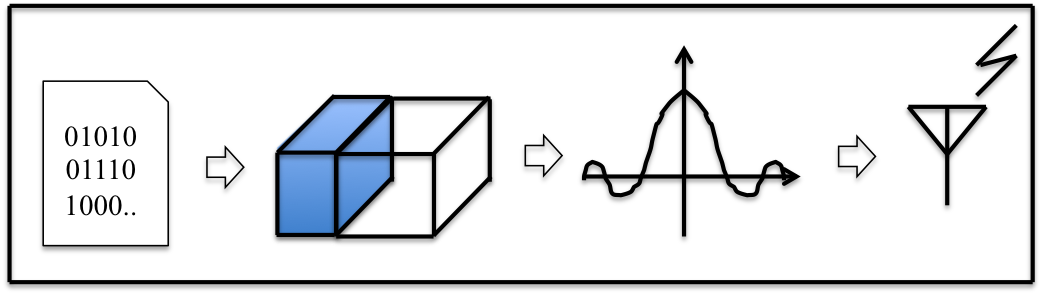
\includegraphics[width=3.1in]{figure/tx.png}
	\caption{TX model}
	\label{fig:TX diagram}
	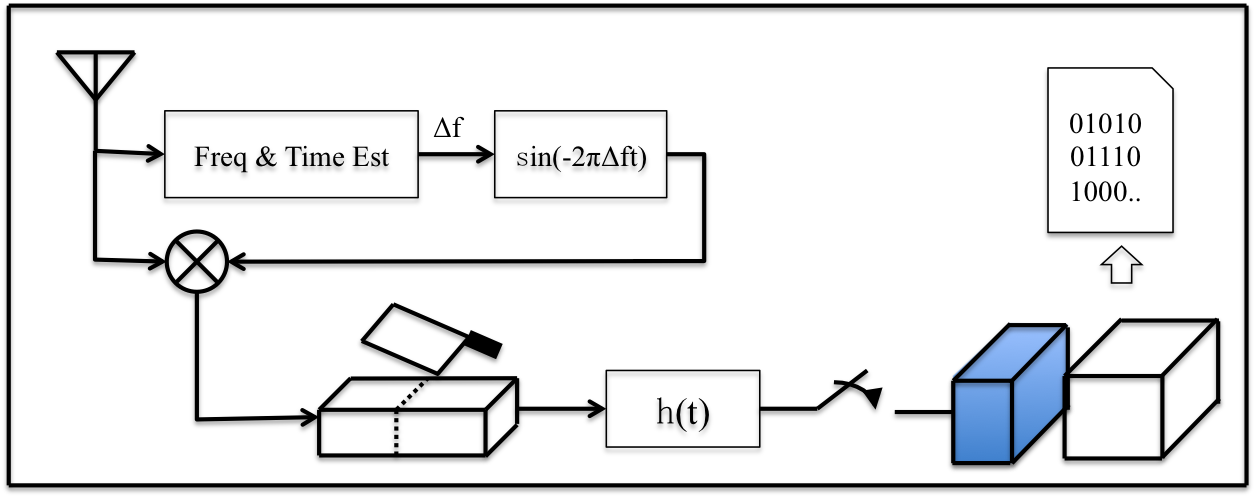
\includegraphics[width = 3.1in]{figure/rx.png}
	\caption{RX model}
	\label{fig:RX diagram}
\end{figure}

From the diagrams, we can see that the complexity of RX model is much more complicated then TX model. The reason is that, the channel will add several uncertainty to the signal, while the transmitter doesn't have to deal with that. So, the main block in the RX model is the ``freq\_\&time\_est'', which will give out the frequency and timing information of the received signal. This article is mainly focus on the performance of this block. 
% section Introduction (end)

\section{Frequency and TIming Trade-off in Estimation}

Trade-off is common in the world. There is one famous theory called uncertainty principle\cite{Uncertainty_Principle}. Also, there is also a trade off for estimating frequency and timing.

In this scenario, we are trying to estimate the frequency offset of the received signal, and estimate the start point of the frame. We will prove that, the estimation cannot be perfect.

\subsection{Mathematical Model} % (fold)
\label{sub:mathematical_model}
The signal we use is $s(t)$:
\begin{align}
	s(t) = 
	\begin{cases}
		\alpha & 0 \leq t \leq T_s\\
		0 	   & else
	\end{cases}
\end{align}
This is a very simple rectangle wave.
For the receiver, we only consider about delay $t_0$ and frequency offset $\Delta f$, the received signal $r(t)$ would be
\begin{align}
	r(t) = s(t - t_0) e^{j 2 \pi \Delta f t}
\end{align}
But for the receiver, it doesn't know anything about the receiver, so the only tag receiver could choose for the matched filter is $h(t)$
\begin{align}
	h(t) = s(T_s - t)
\end{align}
Then, the output of the matched filter is $R(t)$, the result of convolution between $r(t)$ and $h(t)$. 
\begin{align}
	R(t) = r(t) \ast h(t) 
	&= \int_{-\infty}^{+\infty} r(\tau) h(t - \tau) d\tau\\
	&= \int_{t_0}^t s(\tau - t_0)e^{j 2 \pi \Delta f \tau} s(\tau - (t - T_s)) d \tau\\
	&= \int_{t_0}^t \alpha^2 e^{j 2 \pi \Delta f \tau} d \tau\\
	&= \alpha^2 \frac{e^{j 2 \pi \Delta f t}}{j 2\pi \Delta f} \bigg|_{t_0}^t\\
	&= \alpha^2 \frac{e^{j 2\pi \Delta f t} - e^{j 2\pi \Delta f t_0}}{j 2\pi \Delta f}
\end{align}

Now, we will discuss three specific situations:
\subsubsection{$\Delta f = 0$ and $t_0 = 0$} % (fold)
\label{ssub:no freq offset or delay}
We will find that, the numerator and denominator are all 0, so we will turn to L'Hospital.
\begin{align}
	 &\lim_{\Delta f \rightarrow 0} \alpha^2 \frac{e^{j 2\pi \Delta f t} - e^{j 2\pi \Delta f t_0}}{j 2\pi \Delta f}\\
	 =& \lim_{\Delta f \rightarrow 0} \alpha^2 \frac{j 2\pi t e^{j 2\pi \Delta f t} - j 2\pi t_0 e^{j 2\pi \Delta f t_0}}{j 2\pi}\\
	 =& \alpha^2(t - t_0)
\end{align}
When $t_0 = 0$, $R(t) = \alpha^2 t$.
And we know that, because of the domain of $t$, we know that, when $t = T_s$, $R(t)$ will get its maximum value $R(Ts) = \alpha^2 T_s$.

\subsubsection{$\Delta f = 0$, $t_0 = ?$} % (fold)
\label{ssub:no freq offset, but delay is unknown}
Similar to the procedure in part \ref{ssub:no freq offset or delay}, also sample at $t = T_s$
\begin{align}
	R(t) = \alpha^2(T_s-t_0) \Rightarrow \hat{t_0} = T_s - \frac{R(t)}{\alpha^2}
\end{align}

\subsubsection{$t_0 = 0$, but $\Delta f = ?$} % (fold)
\label{ssub:no delay, but freq offset is unknown}
Sample at $t = T_s$
\begin{align}
	R(t) = \alpha^2 \frac{e^{j 2\pi \Delta f T_s} - 1}{j 2\pi \Delta f} = \alpha^2 T_s e^{j \pi \Delta f T_s} sa(\Delta 2 \pi f Ts)
\end{align}
So, we know that, when we get the correct $\Delta f$, we will get the largest value. 

But we still haven't touch the situation where $\Delta f = ?$ and $t_0 = ?$. Our method is brute search.
We enumerate all the possible pair of parameters $(t_0', \Delta f')$, and try them. With the help of above three theory, we know that, the correct/similar to true value will give out the largest $R(t)$.
% subsection mathematical_model (end)

\section{Input Signal of Peak Detector} % (fold)
\label{sec:input_signal_of_peak_detector}
For the ``freq\_timing\_est'' block, frequency and timing information are supposed to be estimated. As discussed in the ``freq\_timing\_tradeoff'', we can use brutal search to get the correct value. But, before we make our decision by choosing the maximum peak, we still need to have a rigorous mathematic model for the peak. 

This section will discuss the mathematic model for ``True'' peak and other points.


\subsection{Mathematical Model} % (fold)
\label{sub:mathematical_model}
Because the signal we received are discrete values, so we only consider about discrete signals, rather than continuous ones.

\begin{table}[ht]
\centering
\begin{tabular}{l l}
 \toprule
 Notation 	& 	Description\\
 \midrule
 $s_k$		& 	received sample at time $k$\\
 $t_k$		& 	training sample at time $k$\\
 $d_k$		& 	data sample at time $k$\\
 $n_k$		& 	noise at time $k$\\
 $P^t_k$ & 	the $k^{th}$ chip of spread code for one frame of training\\
 $P^d_k$	& 	the $k^{th}$ chip of spread code for one frame of data\\
 $D^t_l$ & 	the $l^{th}$ symbol for training\\
 $D^d_l$ & 	the $l^{th}$ symbol for data\\
 $N_f$ 		& 	number of chips per frame\\
 $N_c$ 		& 	number of chips per symbol\\
 $N_s$		& 	number of symbols per frame\\
 $N_{s'}$ 	& 	number of symbols per shortened training sequence\\
 $\sigma^2$ & 	variance of Gaussian noise\\
 $k_0$ 		& 	number of samples of delay\\
 $f_0$ 		& 	frequency offset\\
 $T_c$ 		& 	duration between two chips\\
 \bottomrule
\end{tabular}
\caption{Notation Table}
\label{Table:Notation Table}
\end{table}

First, the structure of training and data frame are like:
The structure of training is like Fig. \ref{fig:Training Frame Structure} and Fig. \ref{fig:Data Frame Structure}
\begin{figure}[ht]
	\centering
	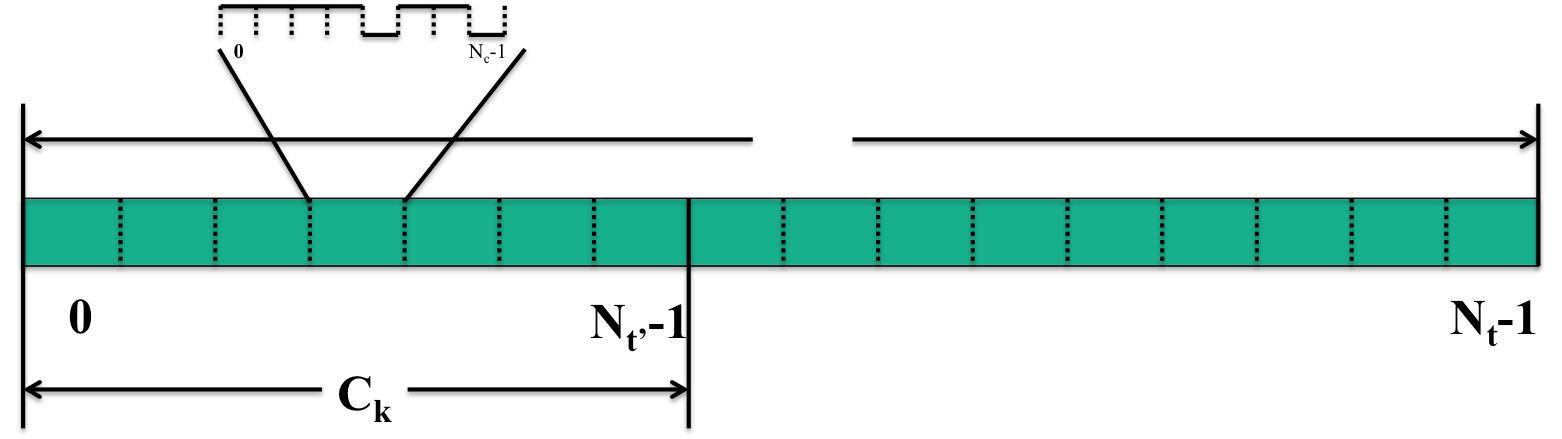
\includegraphics[width = 3.1in]{figure/training_frame.png}
	\caption{Training Frame Structure}
	\label{fig:Training Frame Structure}
	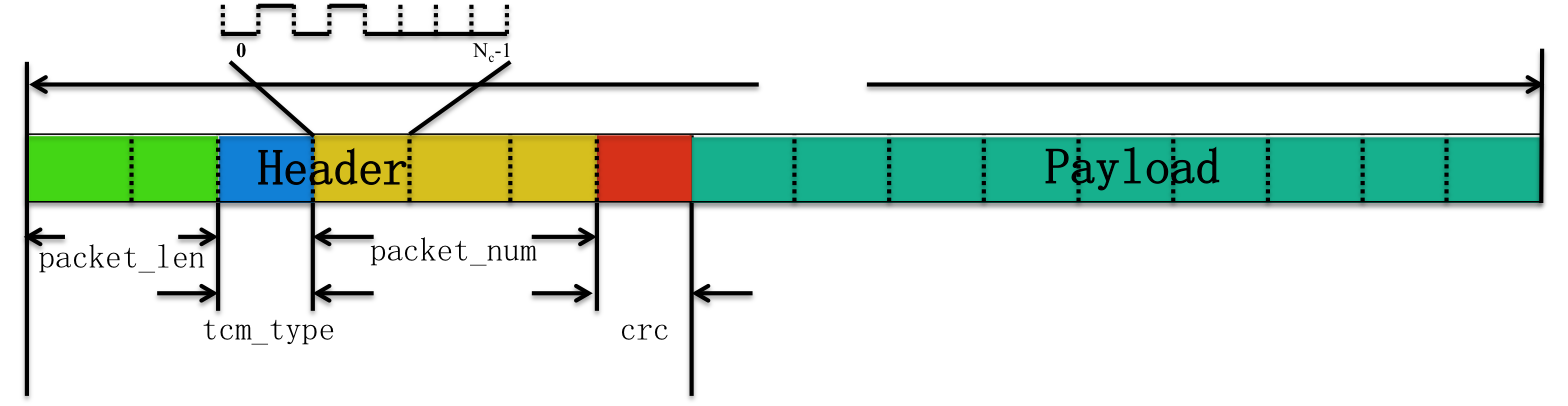
\includegraphics[width = 3.1 in]{figure/data_frame.png}
	\caption{Data Frame Structure}
	\label{fig:Data Frame Structure}
\end{figure}

\subsubsection{Description of Variables} % (fold)
\label{ssub:description_of_variables}
We first express each variables by mathematical languages.

According to the description in table \ref{Table:Notation Table}, and also in order to simplify the following notation, the definition of $P^x_y$ is defined as 
\begin{equation}
\begin{split}
	&P^x_k = 
	\begin{cases}
		P^x_k 	& k = 0, \cdots, N_c-1\\
		0 			& else
	\end{cases}\\
	&x = ``t'' or ``d''
\end{split}
\end{equation}

For instance, the figure for $P^t_k$ is like Fig. \ref{fig:Sketch Map of P_tk}
\begin{figure}
	\centering
	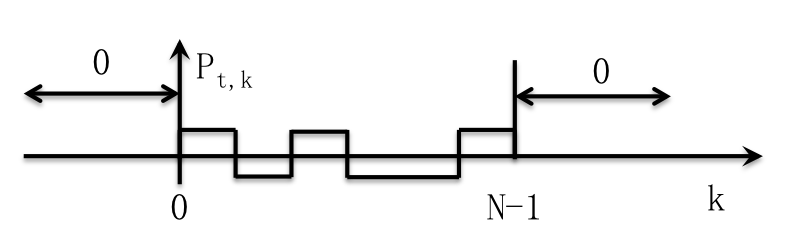
\includegraphics[width = 3.1 in]{figure/p_t_k.png}
	\caption{Sketch Map of $P^t_k$}
	\label{fig:Sketch Map of P_tk}
\end{figure}

So, training chip at time $k$ can be described as:
\begin{align}
		t_k 
	&= \sum_{k = 0}^{N_c} D^t_0 P^t_{k}\\
	&= D^t_0 P^t_k \label{eq:t_k only consider the cyclic property of symbol level}
\end{align}

If we consider the frame-level periodicity, $t_k$ would be
\begin{align}
	t_k = D^t_{\floor{k / N_c} \% N_s} P^t_{k \% N_c}
\end{align}

Based on nearly the same idea, $d_k$ can be written as:
\begin{align}
	d_k = D^d_{\floor{k / N_c}} P^d_{k \% N_c}
\end{align}

Noise is simple. We simply choose IID Gaussian noise. So
\begin{align}
	n_k \sim \mathcal{N}(0, \sigma^2)
\end{align}
% subsubsection description_of_variables (end)

\subsubsection{Description of Output of Matched Filter} % (fold)
\label{ssub:description_of_output_of_matched_filter}
Consider the time delay and frequency offset, the received signal would be 
\begin{align}
	r_k = (t_{k - k_0} + d_{k - k_0}) e^{j 2\pi f_0 k T_c} + n_k
\end{align}

We first deal with the contribution of noise.
Define the Pulse Response of Matched Filter to be $h_{N_f-k}$.
\begin{align}
	h_k = 
	\begin{cases}
	P^t_{k} = D^t_{\floor{k/N_c}}P^t_{k\%N_c} & k = 0, \cdots, N_f\\
	0 	& else	
	\end{cases}
\end{align}
Let $g^n_{k_0}= \sum_{k' = 0}^{N_f-1} n_{k'} \cdot h_{k'}$

\begin{align}
	\mathbb{E} \{ g^n_{k_0}\}
	&= \mathbb{E} \{\sum_{k' = 0}^{N_f-1} n_{k'} \cdot h_{k'}\} \\
	&= \sum_{k' = 0}^{N_f-1} \mathbb{E} \{ n_{k'} \cdot h_{k'} \} \\
	&= \sum_{k' = 0}^{N_f-1} \mathbb{E} \{ n_{k'}\} h_{k'} \\
	&= \sum_{k' = 0}^{N_f-1} 0 \cdot h_{k'} \\
	&= 0\\
	\mathbb{E} \{ (g^n_{k_0})^2\}
	&= \mathbb{E} \{\sum_{k' = 0}^{N_f-1} (n_{k'} \cdot h_{k'}\} \\
	&= \mathbb{E} \{\sum_{k' = 0}^{N_f-1} n_{k'}^2 \cdot \underbrace{(h_{k'})^2}_{\equiv1}\} \\
	&= \sum_{k' = 0}^{N_f-1} \mathbb{E} \{n_{k'}^2 \}\\
	&= N_f \sigma^2
\end{align}

So $g^n_{k_0}\sim \mathcal{N} (0, N_f \sigma^2)$

The next step is to analyze the output of Matched Filter. 
Define the patten for Matched Filter for training frame to be $P^{t*}_{-k}$.
The output of the Matched Filter at sampled point $k=N_f$ is:
\begin{align}
	g_{k_0} 
	&= r_k \ast h_{N_f - k} \bigg|_{k = N_f-1}\\
	&= (t_{k - k_0} + d_{k - k_0} + n_k) \ast h_{N_f -1- k} \bigg|_{k = N_f-1}\\
	&= \underbrace{\sum_{k' = 0}^{N_f-1} t_{k'-k_0}\cdot h_{k'}}_{g^t_{k_0}} + \underbrace{\sum_{k' = 0}^{N_f-1} d_{k'-k_0}\cdot h_{k'}}_{g^d_{k_0}} + \underbrace{\sum_{k' = 0}^{N_f-1} n_{k'}\cdot h_{k'}}_{g^n_{k_0}}\\
	&= g^t_{k_0} + g^d_{k_0} + g^n_{k_0}
	% g_{k_0}
	% &= r_k \ast h_{N_f-k} \bigg|_{k = N_f}\\
	% &= \sum_{k' = 0}^{N_f-1} r_{k'} h_{N_f-(k - k')}\bigg|_{k = N_f}\\
	% &= \sum_{k' = k-N_f+1}^{k} r_{k'} \cdot h_{k' + (N_f-k)}\bigg|_{k = N_f}\\
	% &= \sum_{k' = 0}^{N_f-1} (t_{k'-k_0-N_f+1} + d_{k'-k_0-N_f+1} + n_{k'-k_0-N_f+1}) \cdot h_{k'}\\
	% &= \sum_{k' = 0}^{N_f-1} (t_{k'-k_0-N_f+1} + d_{k'-k_0-N_f+1}) \cdot h_{k'} + \sum_{k' = 0}^{N_f-1} n_{k'-k_0-N_f+1} \cdot h_{k'}\\
	% &= \sum_{k' = 0}^{N_f-1} (t_{k'-k_0-N_f+1} + d_{k'-k_0-N_f+1}) \cdot h_{k'} + \sum_{k' = 0}^{N_f-1} n_{k'} \cdot h_{k'}\\
	% &= \sum_{k' = 0}^{N_f-1}  (t_{k'-k_0-N_f+1} + d_{k'-k_0-N_f+1}) \cdot h_{k'} + g^n_{k}\\
	% &= \underbrace{\sum_{k' = 0}^{N_f-1} t_{k'-k_0-N_f+1} \cdot h_{k'}}_{g^t_{k_0}} + \underbrace{\sum_{k' = 0}^{N_f-1} d_{k'-k_0-N_f+1} \cdot h_{k'}}_{g^d_{k_0}} + g^n_{k_0}\\
	% &= g^t_{k_0}+ g^d_{k_0}+ g^n_{k_0}
\end{align}

Now, we will discuss all the possible situations for timing. 
Let's formate the time offset $k_0$ in terms of $N_s$ and $N_c$.
\begin{align}
	k_0 = \alpha \cdot N_c + \beta ~~~ \alpha = \mathbb{Z}~and~\beta = 0, \cdots, N_c - 1
\end{align}


\paragraph{Perfectly Aligned} % (fold)
\label{par:perfectly_aligned}
Perfectly Aligned means the sample at time $k$ is also the first sample of patten for Matched Filter, as shown in fig. \ref{fig:Perfectly Aligned}.
\begin{figure}[ht]
	\centering
	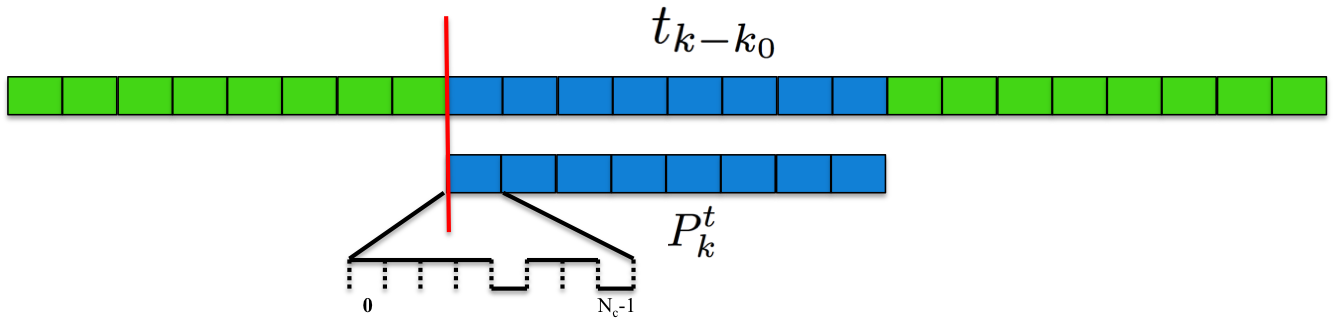
\includegraphics[width=3.1in]{figure/perfectly_aligned.png}
	\caption{Perfectly Aligned}
	\label{fig:Perfectly Aligned}
\end{figure}
For this situation, $k_0$ satisfies 
\begin{align}
	\begin{cases}
		\alpha = z \cdot N_s ~ z \in \mathbb{Z}\\
		\beta = 0
	\end{cases}
	\Rightarrow
	k_0 = z \cdot N_s \cdot N_c
\end{align}

Then we can analyze $g^t_{k_0}$ and $g^d_{k_0}$ separately.

For $g^t_{k_0}$: \label{eq:perfectly aligned-training}
\begin{align}
	g^t_{k_0}
	&= \sum_{k' = 0}^{N_f-1} t_{k'-k_0} \cdot h_{k'}\\
	&= \sum_{k' = 0}^{N_f-1} D^t_{\floor{(k'-k_0) / N_c}\%N_s} P^t_{k' \% N_c} \cdot h_{k'}\\
	&= \sum_{k' = 0}^{N_f-1} D^t_{\floor{(k'-z \cdot N_s \cdot N_c) /N_c}\% N_s} P^t_{k' \% N_c} \cdot h_{k'}\\
	&= \sum_{k' = 0}^{N_f-1} D^t_{\floor{k'/N_c}\%N_s} P^t_{k' \% N_c} \cdot h_{k'}\\
\end{align}
\begin{align}
	\because 
	h_{k'} &= D^t_{\floor{k'/N_c}} P^t_{k' \% N_c}\\
	\therefore
	g^t_{k_0}
	&= \sum_{k' = 0}^{N_f-1} D^t_{\floor{k'/N_c}\%N_s} P^t_{k' \% N_c} \cdot D^t_{\floor{k'/N_c}} P^t_{k \% N_c} \\
	&= \sum_{k' = 0}^{N_f-1} \underbrace{(D^t_{\floor{k'/N_c}\%N_s})^2}_{\equiv 1} \underbrace{(P^t_{k' \% N_c})^2}_{\equiv1}\\
	&= N_f
\end{align}

To analyzie $g^s_k$, we will first define a function to describe the convolution
\begin{align}
	C^n_s(f_1, f_2, k_0) = \sum_{k = s}^{s+n} f_1(k)\cdot f_2(k - k_0) \label{eq:New Defined Convolution}
\end{align}

The diagram of the above formula is like Fig.\ref{fig:New Defined Convolution}
\begin{figure}[ht]
	\centering
	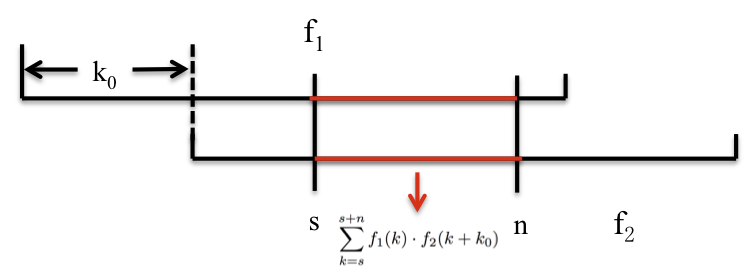
\includegraphics[width=3.1in]{figure/conv_figure.png}
	\caption{New Defined Convolution}
	\label{fig:New Defined Convolution}
\end{figure}
Then $g^d_{k_0}$: \label{eq:perfectly aligned-data}
\begin{align}
	g^d_{k_0}
	&= \sum_{k' = 0}^{N_f-1} d_{k' - k_0} \cdot h_{k'} \\
	&= \sum_{k' = 0}^{N_f-1} D^d_{\floor{(k' - k_0)/N_c}}P^d_{(k' - k_0)\%N_c} \cdot h_{k'}\\
	&= \sum_{k' = 0}^{N_f-1} D^d_{\floor{(k' - z \cdot N_s \cdot N_c)/N_c}} P^d_{(k' - z \cdot N_s \cdot N_c)\%N_c}\cdot h_{k'}\\
	&= \sum_{k' = 0}^{N_f-1} D^d_{\floor{k'/N_c} - z \cdot N_s} P^d_{k'\%N_c} \cdot D^t_{\floor{k'/N_c}} P^t_{k' \% N_c} 
\end{align}
For data symbols, we could only assume that 
\begin{align}
	D^d_k = 
	\begin{cases}
	+1 & p = 0.5\\
	-1 & p = 0.5	
	\end{cases}
\end{align}
Because the $D^d_k$ here is a random variable, we could only exam the mean and variance for it, so do the $g^d_{k_0}$
\begin{align}
	&\mathbb{E} \{D^d_k\} = 1 \times 0.5 + (-1) \times 0.5 = 0\\
	&\mathbb{E} \{D^d_k)^2\} = 1 \times 0.5 + (-1)^2 \times 0.5 = 1
\end{align}
and they are IID.

For $g^d_{k_0}$,

\begin{align}
	% mean
	\mathbb{E} \{g^d_{k_0}\} 
	&= \mathbb{E} \{\sum_{k' = 0}^{N_f-1} D^d_{\floor{k'/N_c} - z \cdot N_s} P^d_{k'\%N_c} \cdot D^t_{\floor{k'/N_c}} P^t_{k' \% N_c}\}\\
	&= \sum_{k' = 0}^{N_f-1} \mathbb{E}\{ D^d_{\floor{k'/N_c} - z \cdot N_s} P^d_{k'\%N_c} \cdot D^t_{\floor{k'/N_c}} P^t_{k' \% N_c}\}\\
	&= \sum_{k' = 0}^{N_f-1} P^d_{k'\%N_c} P^t_{k' \% N_c} \mathbb{E} \{ D^d_{\floor{k'/N_c} - z \cdot N_s} D^t_{\floor{k'/N_c}}\}\\
	&= C_0^{N_c-1}(P^d_{k}, P^t_{k}, 0) \sum_{k'' = \floor{k'/N_c}}^{\floor{k'/N_c} + N_s - 1} D^t_{k''}\mathbb{E} \{ D^d_{k'' - z} \}\\
	&= 0
\end{align}
\begin{align}
	% variance
	\mathbb{E} \{(g^d_{k_0})^2\}
	&= \mathbb{E} \{\sum_{k' = 0}^{N_f-1} D^d_{\floor{k'/N_c} - z \cdot N_s} P^d_{k'\%N_c} \cdot D^t_{\floor{k'/N_c}\%N_s} P^t_{k \% N_c}\}^2\\
	&= \mathbb{E} \{\sum_{k'' = \floor{k'/N_c}}^{\floor{k'/N_c} + N_s - 1} D^t_{k''} D^d_{k'' - z} \cdot \sum_{m = 0}^{N_c} P^d_{m\%N_c} P^t_{m \% N_c} \}^2\\
	&= \big(\sum_{m = 0}^{N_c} P^d_{m} P^t_{m }\big)^2 \mathbb{E} \{\sum_{k'' = \floor{k'/N_c}}^{\floor{k'/N_c} + N_s - 1} D^t_{k''} D^d_{k'' - z}\}^2\\
	&= (C_0^{N_c-1}(P^d_{k}, P^t_{k}, 0))^2 \mathbb{E}\{\sum_{k'' = \floor{k'/N_c}}^{\floor{k'/N_c} + N_s - 1} D^t_{k''} D^d_{k''}\}^2\\ 
	\begin{split}
		&=(C_0^{N_c-1}(P^d_{k}, P^t_{k}, 0))^2 \bigg(\mathbb{E} \{\sum_{m = \floor{k'/N_c}}^{\floor{k'/N_c} + N_s - 1} (D^t_{m} D^d_{m})^2\}\\
		&+ \mathbb{E} \{ \sum_{m = \floor{k'/N_c}}^{\floor{k'/N_c} + N_s - 1} \sum_{n \neq m} D^t_{m} D^d_{m} D^t_{n} D^d_{n}\} \bigg)
	\end{split}\\
	\begin{split}
		&= (C_0^{N_c-1}(P^d_{k}, P^t_{k}, 0))^2 \bigg( \sum_{m = \floor{k'/N_c}}^{\floor{k'/N_c} + N_s - 1} \mathbb{E} \{ D^d_{m}\}^2\\
		&+ \sum_{m = \floor{k'/N_c}}^{\floor{k'/N_c} + N_s - 1} \sum_{n \neq m} D^t_{m} D^t_{n} \mathbb{E} \{D^d_{m}\} \mathbb{E} \{D^d_{n}\} \bigg)
	\end{split}\\
	&= (C_0^{N_c-1}(P^d_{k}, P^t_{k}, 0))^2 \bigg( \sum_{m = \floor{k'/N_c}}^{\floor{k'/N_c} + N_s - 1} \cdot 1 \bigg)\\
	&= (C_0^{N_c-1}(P^d_{k}, P^t_{k}, 0))^2 \cdot N_s
\end{align}
% paragraph perfectly_aligned (end)


% paragraph  (end)
\paragraph{Chip-level Aligned} % (fold)
\label{par:chip_level_aligned}
Chip-level Aligned means the start chip of received symbol is aligned with patten's symbol's first chip. But, the begining symbol of a frame for received data may not be aligned with patten's first symbol. Here is the diagram
\begin{figure}[ht]
	\centering
	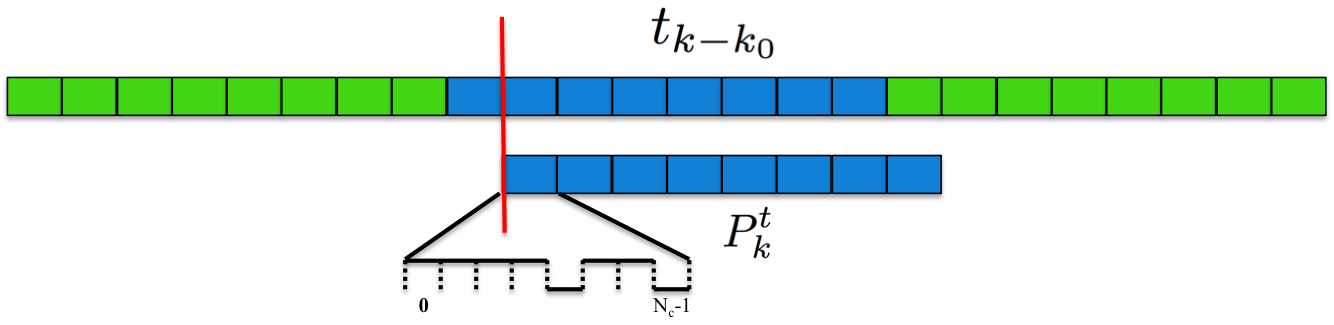
\includegraphics[width = 3.1in]{figure/chip_level_aligned.png}
	\caption{Chip-level Aligned}
	\label{fig:Chip-level aligned}
\end{figure}

At this time
\begin{align}
	\begin{cases}
		\alpha = z &z \in \mathbb{Z}\\
		\beta = 0 &
	\end{cases}
	\Rightarrow k_0 = z \cdot N_c
\end{align}

For $g^t_{k_0}$: \label{eq:chip-level aligned-training}
\begin{align}
	g^t_{k_0}
	&= \sum_{k' = 0}^{N_f-1} t_{k'-k_0} \cdot h_{k'}\\
	&= \sum_{k' = 0}^{N_f-1} D^t_{\floor{(k'-k_0) / N_c}\%N_s} P^t_{k \% N_c} \cdot h_{k'}\\
	&= \sum_{k' = 0}^{N_f-1} D^t_{\floor{(k'-z \cdot N_c) / N_c}\%N_s} P^t_{k \% N_c} \cdot D^t_{\floor{k'/N_c}} P^t_{k \% N_c}\\
	&= \sum_{k' = 0}^{N_f-1} D^t_{(\floor{k' / N_c} - z)\%N_s} D^t_{\floor{k'/N_c}} \underbrace{P^t_{k \% N_c} P^t_{k \% N_c}}_{\equiv 1}\\
	&= \sum_{k' = 0}^{N_f-1} D^t_{(\floor{k' / N_c} - z)\%N_s} D^t_{\floor{k'/N_c}}\\
	&= C_z^{N_s-1}(D_k^t, D_k^t, z) + C_{N_s - z}^{N_s-1}(D_k^t, D_k^t, N_s - z)
\end{align}
\begin{figure}[ht]
	\centering
	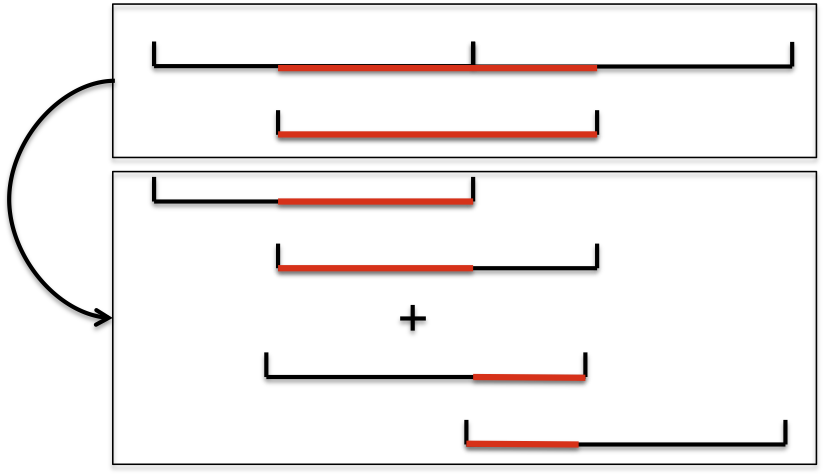
\includegraphics[width=3.1in]{figure/misaligned_conv.png}
	\caption{Diagram for Misaligned Convolution}
	\label{fig:Diagram for Misaligned Convolution}
\end{figure}

For $g^d_{k_0}$: \label{eq:chip-level aligned-data}
\begin{align}
	% mean
	\mathbb{E} \{g^d_{k_0}\} 
	&= \mathbb{E} \{\sum_{k'=0}^{N_f-1} D^d_{\floor{k'/N_c}-z} P^d_{k'\%N_c} \cdot D^t_{\floor{k'/N_c}\%N_s} P^t_{k\%N_c} \}\\
	&= \sum_{k'=0}^{N_f-1} \mathbb{E} \{ D^d_{\floor{k'/N_c}-z} P^d_{k'\%N_c} \cdot D^t_{\floor{k'/N_c}\%N_s} P^t_{k\%N_c} \}\\
	&= \sum_{m = 0}^{N_c} (P^d_{m} P^t_{m}) \sum_{m = \floor{k'/N_c}}^{\floor{k'/N_c}+N_s-1} D^t_{m} \mathbb{E}\{ D^d_{m-z} \}\\
	&= C_0^{N_c}(P_k^d, P_k^t, 0) \cdot \sum_{m = \floor{k'/N_c}}^{\floor{k'/N_c}+N_s-1} D^t_{m} \cdot0\\
	&= 0
\end{align}
\begin{align}
	% variance
	\mathbb{E} \{(g^d_{k_0})^2\}
	&= \mathbb{E} \{\sum_{k'=0}^{N_f-1} D^d_{\floor{k'/N_c}-z} P^d_{k'\%N_c} \cdot D^t_{\floor{k'/N_c}\%N_s} P^t_{k\%N_c} \}^2\\
	&= (C_0^{N_c}(P_k^d, P_k^t, 0))^2 \mathbb{E}\{\sum_{m = \floor{k'/N_c}}^{\floor{k'/N_c}+N_s-1} D_{m-z}^t D_{m}^d \}^2\\
	&= (C_0^{N_c}(P_k^d, P_k^t, 0))^2 \mathbb{E}\{\sum_{m = \floor{k'/N_c}}^{\floor{k'/N_c}+N_s-1} D_{m}^t D_{m}^d \}^2\\
	&= (C_0^{N_c-1}(P^d_{k}, P^t_{k}, 0))^2 \cdot N_s
\end{align}

The mean and variance of $g^d_{k_0}$ is the same as the situation of perfectly aligned.
% paragraph chip_level_aligned (end)

\paragraph{Totally Misaligned} % (fold)
\label{par:totally_misaligned}
Totally Misaligned means the first chip of received data is not correspond to the first chip of patten. Like the Fig. \ref{fig:Totally Misaligned}
\begin{figure}[ht]
	\centering
	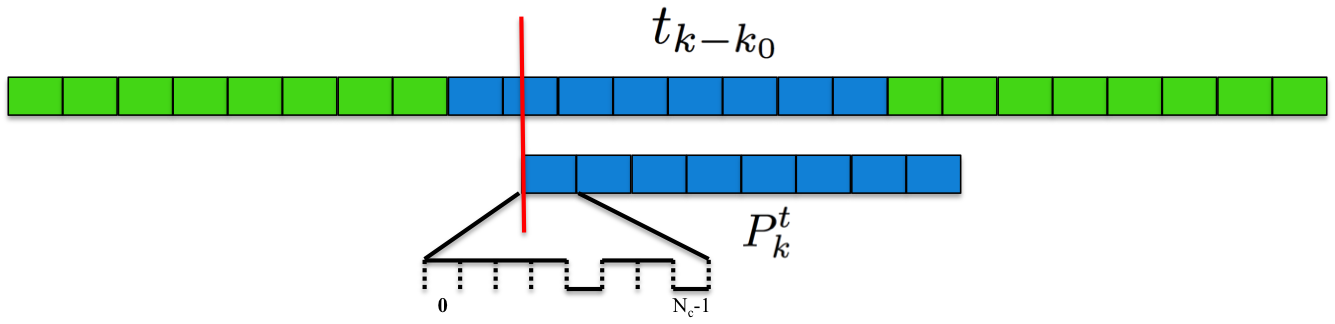
\includegraphics[width = 3.1in]{figure/totally_misaligned.png}
	\caption{Totally Misaligned}
	\label{fig:Totally Misaligned}
\end{figure}

\begin{align}
	k_0 = z, ~ z\in \mathbb{Z}
\end{align}

For $g_{k_0}^t$: \label{eq:totally misaligned-training}
\begin{align}
	g^t_{k_0} 
	&= \sum_{k' = 0}^{N_f-1} t_{k' - k_0} \cdot h_{k'}\\
	&= \sum_{k' = 0}^{N_f-1} D^t_{\floor{(k'-z)/N_c}\%N_s} P^t_{(k'-z)\% N_c} \cdot D^t_{\floor{k'/N_c}} P^t_{k\%N_c}
\end{align}

We will first deal with a smaller problem. If we only focus on patten of length $N_c$
\begin{figure}[ht]
	\centering
	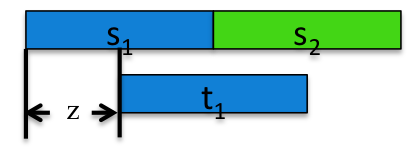
\includegraphics[width = 3.1in]{figure/chip_level_misaligned.png}
	\caption{Chip-level Misaligned}
	\label{Chip-level Misaligned}
\end{figure}
Define the result of the above situation to be $f^t(s_1, s_2, t_1, z)$
\begin{align}
	f^t(s_1, s_2, t_1, z) = (s_1 \cdot t_1)C_z^{N_c-1}(P^t_{k}, P^t_{k}, z) + (s_2 \cdot t_1) C_{N_c - z}^{N_c-1}(P^t_{k}, P^t_{k}, N_c - z)
\end{align}
Now, back to $g^t_{k_0}$ \label{eq:totally misaligned-training}
\begin{align}
	g^t_{k_0}
	&= \sum_{m = \floor{(-k_0)/N_c}, n = 0}^{\floor{m=(-k_0)/N_c} + N_s, n = N_s} f^t_{m\%N_s, m+1\%N_s, n, z\%N_c}
\end{align}

For $g^d_{k_0}$ \label{eq:totally misaligned-data}
\begin{align}
	\mathbb{E} \{g^d_{k_0}\} 
	&= \sum_{k' = 0}^{N_f-1} D^d_{\floor{(k'-z)/N_c}\%N_s} P^d_{(k'-z)\% N_c} \cdot D^t_{\floor{k'/N_c}} P^t_{k\%N_c}
\end{align}

We can also define
\begin{align}
	f^d_1(s_1, s_2, t_1, z) = (s_1 \cdot t_1)C_z^{N_c-1}(P^d_{k}, P^t_{k}, z) + (s_2 \cdot t_1) C_{N_c - z}^{N_c-1}(P^d_{k}, P^t_{k}, N_c - z)
\end{align}

Then $g_{k_0}^d$ would be 
\begin{align}
	g^d_{k_0}
	&= \sum_{m = \floor{(-k_0)/N_c}, n = 0}^{\floor{m=(-k_0)/N_c} + N_s, n = N_s} f^d(m, m+1, n, z\%N_c)
\end{align}
But for the expectation, we may need to change a little bit. Because we want to split the patten symbol rather than the received symbol.
\begin{align}
	g^d_{k_0}
	&= \sum_{m = \floor{(-k_0)/N_c}, n = 0}^{\floor{m=(-k_0)/N_c} + N_s, n = N_s} f^d(n, n+1, m, z\%N_c)
\end{align}
Then
\begin{align}
	\mathbb{E}\{g^d_{k_0}\} 
	&= \mathbb{E}\{\sum_{m = \floor{(-k_0)/N_c}, n = 0}^{\floor{m=(-k_0)/N_c} + N_s, n = N_s} f^d(n, n+1, m, z\%N_c)\}\\
	&= \sum_{m = \floor{(-k_0)/N_c}, n = 0}^{\floor{m=(-k_0)/N_c} + N_s, n = N_s} \mathbb{E}\{f^d(n, n+1, m, z\%N_c)\}\\
	&= 0
\end{align}
\begin{align}
	\mathbb{E} \{(g^d_{k_0})^2\}
	&= \bigg(C_{z\%N_c}^{N_c-1}(P^d_k, P^t_k, z\%N_c) + C_0^{z-1}(P^d_k, P^t_k, -z\%N_c)\bigg)^2 \cdot N_s
\end{align}

Because we can view it as a shifted training patten.


\subsubsection{Ideal Situation} % (fold)
\label{ssub:ideal_situation}

The formulas above are for practical situations. For idea situations, we would like to let spread codes have properities like below:

\begin{enumerate}
	\item Different spread codes are orthogonal;
	\item Autocorrelation is a $\delta$ function.
\end{enumerate}

So the auto-correlation and cross-correlation are like:

\begin{figure}[ht]
	\centering
	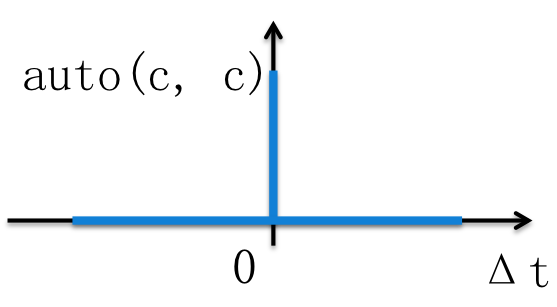
\includegraphics[width = 3.1in]{figure/autocorrelation.png}
	\caption{Auto-correlation for certain spread codes}
	\label{fig:auto-correlation}
	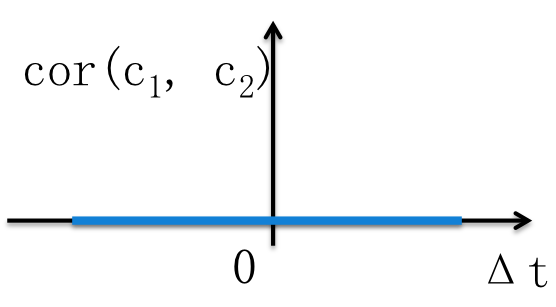
\includegraphics[width = 3.1in]{figure/cross-correlation.png}
	\caption{Cross-correlation for different spread codes}
	\label{fig:cross-correlatino}
\end{figure}

The mathematical description for this property would be:
\begin{align}
	&\text{for different spread codes }C_i(t) \text{and} C_j(t), i \neq j \text{means they are different.} \nonumber\\
	&c_i(t) \ast c_i(-t + \Delta t) = 
	\begin{cases}
		N_c &	\Delta t = k \cdot N_c, k = \mathbb{Z}\\
		0 	& 	else
	\end{cases}\\
	&c_i(t) \ast c_j(-t + \Delta t) = 0, \forall k \in \mathbb{Z}
\end{align}

Compared the ideal situation with the analysis did in subsection \ref{ssub:description_of_output_of_matched_filter}, because the spread code for training and data are orthogonal, or say different, so 

\begin{align}
	g^d_{k_0} \equiv 0
\end{align}

Because the auto-correlation function has perfect property, eq \ref{eq:chip-level aligned-training} and eq \ref{eq:totally misaligned-training} should be as close to 0 as possible.

\chapter{Acknowledge}
Should you have any questions about this documents, feel free to talk or email me. Because I finished this document in a hurry, I am sure that I must ignore some parts and make dozens of mistakes. Please point out them for me, thank you very much!
We would also like to thank every contributor who has ever devoted time to this project. 

\bibliographystyle{plain}
\bibliography{bibliography.bib}

\end{document}
